\documentclass[11pt,openany,twoside]{report}
\usepackage[utf8]{inputenc}
\usepackage[hmargin=4cm,vmargin=3.5cm,bmargin=3.5cm]{geometry}
\usepackage[portuguese, english]{babel}
\usepackage{graphicx}
\usepackage{hyperref}
\usepackage{indentfirst}

\title{\textbf{Projeto 2 - Descrição dos módulos}}

\begin{document}

\begin{titlepage}
\begin{figure}
\title{\textbf{Projeto 2 - Descrição dos módulos}}
\author{\\\vspace{0.3cm}
Abel Fernandes Neto
\\\vspace{0.3cm}
Daniel Azevedo Alves
\\\vspace{0.3cm}
Diogo Daniel Soares Ferreira
\\\vspace{0.3cm} 
Luís Davide Jesus Leira
\\\vspace{0.3cm}
\textbf{Universidade de Aveiro - Laboratórios de Informática - Grupo 3}}
\date{\today}
 
\includegraphics[scale=1.5]{ua_logo.png}
\end{figure}
\end{titlepage}

\selectlanguage{portuguese}
\maketitle
\tableofcontents
\listoffigures

\part{Apresentação}

\chapter{Resumo}
Neste relatório são descritos os passos necessários e a divisão do trabalho para a realização do projeto 2 de Laboratórios de Informática. O projeto consiste sucitamente numa aplicação Web capaz de receber uma pauta no formato \textit{RTTTL} (\textit{RingTone Text Transfer Language}), sendo possível aplicar registos e efeitos, dando origem a uma música. Será possível obter o seu gráfico das notas e o ficheiro áudio, cuja sonoridade se assemelha a um orgão \textit{Hammond}, daí o nome da aplicação \textit{Virtual Hammond}. Deverá ser concluído e enviado até dia 7 de Junho de 2015. Os desenvolvedores utilizam o repositório do \textit{CodeUA} (labi2015-proj2-g3) como meio de desenvolvimento deste projeto.

\chapter{Introdução}
As aplicações Web são sistemas de informação onde o utilizador interage com uma página web. Estas encontram-se alojadas em servidores e são apresentadas através de um navegador (vulgarmente conhecido como \textit{browser}). A sua principal função é receber solicitações por parte do cliente, efetuando internamente uma resposta adequada ao pedido, a qual é recebida e mostrada através do navegador. As aplicações Web devem visam pelar simplicidade e pelo cumprimento de tarefas de forma direta.

É pretendido desenvolver uma aplicação web em que permita que seja fornecida uma especificação de uma música no formato \textit{RTTTL} e a sua configuração de registos, dando origem à música correspondente. Toda a informação deverá ser guardada e gerida com recurso a uma base de dados, permitindo ao utilizador ouvir repetidamente as músicas já criadas na aplicação.


\begin{figure}
 \center
 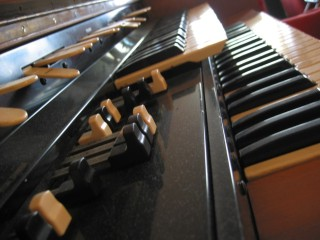
\includegraphics[scale=.4]{Hammond_l100.jpg}
 \caption{Órgão de \textit{Hammond}. Fonte: Wikipédia}
 \label{hammond}
\end{figure}

A aplicação será faseada e dividida de forma equilibrada pelos elementos do grupo. Irá dividir-se na interface web, na aplicação principal em si, no interpretador de pautas e no sintetizador que irá reproduzir as músicas cujo som se pretende que seja semelhante a um orgão de \textit{Hammond} (\autoref{hammond}). Depois, caso esteja tudo funcional e implementado corretamente, será adicionado um processador de efeitos, o qual irá aplicar efeitos de forma individual ou global e originar um ficheiro \textit{WAVE} que será posteriormente armazenado no sistema de ficheiros pertencente à aplicação.

\part{Desenvolvimento}


\chapter{Descrição dos módulos}

\section{Descrição sumária acerca dos módulos}
A interface Web deverá assegurar o aspeto da aplicação e a interação com computadores pessoais e dispositivos móveis. Servirá como meio de transporte e visualização de informação por parte da aplicação principal, apresentando quatro funcionalidades principais que serão detalhadas a seguir. Esta tarefa ficará a cargo do Luís Leira, que se pretende concluída na sua totalidade até dia 31 de Maio.

A aplicação principal servirá de elo de ligação entre os diferentes módulos. Deverá receber os pedidos e instruções do utilizador, através da interface Web, e encaminhar a informação para os módulos a executar. Esta tarefa ficará a cargo do Daniel Alves e deverá ser concluída até 31 de Maio.

O interpretador de pautas deverá, na função \textit{inter}, receber da aplicação principal a pauta, e enviar a sua resposta novamente para a aplicação principal. Esta função ficará a cargo do Diogo Ferreira, que terá até dia 17 de Maio para a completar. Após essa data, deverá ajudar os seus colegas no necessário.

O sintetizador deverá receber uma lista de frequências e transformá-las no formato correto para depois poder ser processado corretamente pelo processador de efeitos. Deverá ser realizado por Abel Neto até dia 17 de Maio. Após essa data, deverá ajudar os seus colegas no necessário.

Caso tudo o que foi anteriormente referido esteja implementado corretamente, será adicionado o processador de efeitos que deverá receber do sintetizador uma lista com as frequências e o nome de um efeito e deverá aplicar esse efeito à lista recebida. Será também gerado um ficheiro \textit{wav} com a música e os efeitos aplicados, que será armazenado no sistema de ficheiros.

\section{Interface Web}
A interface Web é a componente visível e que torna acessível a realização de pedidos de forma a obter uma resposta que provém da interação com a aplicação principal e restantes módulos complementares, sendo a sua visualização ao utilizador da responsabilidade da interface Web. Esta apresenta uma interface simples, a qual contém uma barra superior que se destina para o título e uma hiperligação onde se apresentam os desenvolvedores da aplicação e uma barra inferior que tem a função de \textit{menu} com as seguintes três opções: \textit{Home}, \textit{New music} e \textit{Show all}.

A página inicial é a \textit{Home}, a qual serve de página introdutória à aplicação Web.

A página \textit{New music} permite a criação de uma nova música, onde é pedido o nome da música que se deseja criar, a pauta em formato \textit{RingTone
Text Transfer Language} (RTTTL), o registo e os efeitos a aplicar. O botão \textit{Add song} comunica com a função \textit{createSong} da aplicação principal, recebendo os argumentos e desencadeando uma resposta do sucesso do pedido.

A página \textit{Show all} possibilita diversas ações, entre as quais se verifica prontamente a listagem das músicas presentes na aplicação, isto devido à função \textit{listSongs} da aplicação principal. Assim, é possível efetuar diversos pedidos a cada música, tais como a obtenção da pauta da música, a criação de uma nova interpretação da música em questão e a listagem de todas as versões de uma música (através do botão \textit{Show versions}). Na primeira opção, é devolvida a pauta da música através da interação com o botão \textit{Get notes} o qual irá interagir com a função \textit{getNotes} da aplicação principal. Na opção seguinte, através do botão \textit{New version} é possível criar uma versão com novos registos e/ou efeitos, servindo-se da função \textit{createInterpretation}. É devolvida, também, uma mensagem de sucesso da operação. Na última opção, a listagem é obtida através da função \textit{listSongFiles}, sendo possível escolher uma determinada versão e obter informações e outros conteúdos adicionais, tais como a obtenção de um ficheiro áudio e uma imagem que apresenta o gráfico das notas, os registos, os efeitos aplicados, os votos positivos e negativos dessa interpretação e consequentemente a possibilidade do utilizador votar.

\section{Aplicação principal}
A aplicação principal centraliza as funções de encaminhamento e resposta aos pedidos por parte da interface Web. Para garantir esta resposta recorre-se ao módulo \textit{Cherrypy} e à especificação de funções que respondem a pedidos específicos. A informação passada pelo utilizador à aplicação é guardada numa base de dados, constituída por duas tabelas: \textit{musics} e \textit{interpretations}. A primeira guarda a informação do nome e pauta das músicas. A segunda guarda informação sobre as diferentes interpretações, através dos atributos registos, efeitos sonoros e votos positivos e negativos. Para garantir a ligação entre as tabelas é definido como \textit{foreign key} o atributo \textit{ID} da tabela \textit{musics}.

A estrutura responsável por dar respostas à interface Web é constituída por nove funções, cada uma com uma tarefa específica. As duas primeiras funções são \textit{createSong} e \textit{createInterpretation}, cujas tarefas são a criação de entradas nas tabelas da base de dados. A primeira é acionada sempre que o utilizador pretende criar uma nova música e recebe como argumentos os parâmetros \textit{name} e \textit{notes}, \textit{register} e \textit{effects}, todos na forma de \textit{strings}. Estando o utilizador a criar uma música é necessário criar uma entrada na tabela \textit{musics} e outra na tabela \textit{interpretations}. Esta última é conseguida através do redirecionamento para a função \textit{createInterpretation}. Esta função recebe como argumentos o \textit{ID} da música na forma de número inteiro e o registo e efeitos na forma de \textit{strings}. No caso do utilizador optar pela criação de uma nova versão a partir de uma música existente esta função é ativada diretamente. Tal como na anterior, é criada uma entrada na base de dados com a indicação dos parâmetros recebidos. Não tendo estas funções tarefas de apresentação de ficheiros, a devolução através do \textit{return} é uma mensagem a confirmar o sucesso da operação.

Para que o utilizador possa utilizar músicas existentes na base de dados e consultar as suas informações existem as funções \textit{listSongs} e \textit{listSongFiles}. A apresentação de todas as músicas presentes na base de dados é conseguida com a função \textit{listSongs}. Como não especifica música em particular, não necessita de argumentos. A sua implementação baseia-se na pesquisa e ordenação da informação de todas as músicas presentes na base de dados. Esta informação é constituída pelo \textit{ID} da música e nome da música e é comunicada ao elemento \textit{Javascript} da interface Web, através do formato \textit{JSON}. A função \textit{listSongFiles} tem o objetivo mais específico de apresentar a informação de uma música em particular. Recebe como argumentos o \textit{ID} da música, que usa para fazer a pesquisa na tabela \textit{interpretations} e devolve a informação sobre nome, registos, efeitos sonoros e \textit{ID} das interpretações da música.

Outra função de pesquisa na base de dados é a \textit{getNotes}. O seu objetivo é a pesquisa e devolução da pauta de uma música. Necessita apenas de um argumento, o \textit{ID} da música, que é usado na pesquisa efetuada na tabela \textit{musics} da base de dados. A informação é devolvida no formato \textit{JSON} para o elemento \textit{Javascript} da interface Web.

A interface Web permite a atribuição de votos às interpretações. A informação relativa a estes dados é guardada na tabela \textit{interpretations}. Os votos que podem ser negativos ou positivos são apresentados na página recorrendo à função \textit{showVotes}. Para tal recebe como argumento o \textit{ID} da interpretação que usa para pesquisar a votação na base de dados. A devolução acontece pelo formato \textit{JSON}, com a indicação do número de votos negativos e positivos. O utilizador pode dar a sua opinião carregando nos botões de voto negativo ou positivo. Isto aciona a função \textit{newVotes} que recebe os parâmetros \textit{ID} da interpretação, voto positivo e voto negativo. Cada clique define um valor unitário para o voto positivo ou negativo consoante o botão escolhido. Na tabela \textit{interpretations} é efetuada a atualização da contagem dos votos, sendo devolvidos à página os valores atualizados.

A aplicação desenvolvida permite o acesso a ficheiros áudio das interpretações criadas e a gráficos com a visualização das notas. Na aplicação principal estas tarefas são realizadas pelas funções \textit{getWaveFile} e \textit{getWaveForm} que recebem como argumento o \textit{ID} da interpretação. A função \textit{getWaveFile} pesquisa a pauta da música e passa-a como argumento ao interpretador de pauta, cujo resultado, em conjunto com o registo definido pelo utilizador, é aplicado no sintetizador que cria uma lista de samples para a música. O processador é o último passo na cadeia e é acionado pelo sintetizador, aceitando a lista de sons gerados e os efeitos escolhidos. Depois de aplicados os efeitos, o ficheiro \textit{WAVE} gerado é disponibilizado ao utilizador através da devolução da localização no sistema de ficheiros. A função \textit{getWaveForm} inicia o processo com a procura da pauta que, tal como na função anterior, é usada pelo interpretador de pauta para criar a lista de tuplos (tempo, frequência) usada como argumento na função \textit{createForm}. Esta gera a partir dos valores dados um gráfico representativo das notas presentes na música. Para a criação do gráfico recorre-se ao módulo \textit{matplotlib}. A localização do ficheiro é devolvida, através do formato \textit{JSON} à interface Web, para disponibilização ao utilizador.

\section{Interpretador de pautas}
O interpretador de pautas deverá ter uma função \textit{inter}, que recebe um texto com a pauta no seu formato válido. Caso isso não aconteça, retorna uma lista sem valores. Caso a sua entrada seja válida, irá calcular a duração de cada nota e a frequência, e retornar um lista no formato (duração, frequência) para cada nota descrita. Excecionalmente, a frequência terá o valor da nota recebida, mas duas oitavas abaixo. Isto deve-se ao facto do formato \textit{RTTTL} ser otimizado para telemóveis antigos, e não para uma aplicação \textit{web}, logo foi baixada a frequência para o som ficar mais agradável.

\section{Sintetizador}
O sintetizador tem como objetivo representar digitalmente amostras de um som em sinal analógico. Esta função presente no ficheiro \textit{sint.py} recebe um conjunto de notas com respetiva frequência e duração. Esses dados permitirão construir a forma de onda do sinal analógico e assim proceder à amostragem do mesmo.

O sintetizador recebe também um registo com nove algarismos correspondentes aos nove osciladores do orgão. De notar que o código implementado verifica se este dado de entrada corresponde ao pretendido.

Assim, a função \textit{sintetizador} cria uma lista \textit{enddata} de dicionários \textit{info} com as entradas \textit{freq} e \textit{samples} que indicam a frequência da nota original e os valores de amostragem, respectimente.

Cada dicionário é preenchido através de um ciclo onde é verificada a frequência da nota e a sua duração e através da \autoref{F1} encontramos um a um os valores da amostragem digital do sinal de onda original da nota.

\begin{equation}
 \displaystyle\sum_{j=1}^{9} amplitude * \frac{reg[j]}{8} * \sin(\frac{2*\Pi*f*mul[j]*i}{rate})
 \label{F1} 
\end{equation} 

Os valores \textit{reg} e \textit{mul} representam listas com os dados de registos fornecidos ao sintetizador e a lista de multiplicidade respetivamente. O valor \textit{i} é usado pelo ciclo principal que preencherá a lista \textit{samples} com os valores de sinal digital encontrados pela \autoref{F1}.

Cada lista \textit{samples}, ou digamos cada \textit{frame} será sujeita a um teste que eliminará o efeito de \textit{cliping}.

\section{Processador de efeitos}
O processador de efeitos deverá ter cinco funções que poderá aplicar à sua lista de entrada. A função \textit{echo} somará o sinal atual a um sinal futuro atenuado. A \textit{tremolo} deverá fazer variar o sinal numa amplitude pequena. A distorção deverá elevar o sinal atual a um valor n, sendo que depois os valores devem ser limitados entre -32768 e 32767. A percussão deverá adicionar um múltiplo da frequência da nota, com uma amplitude a decair ao longo do tempo, até se anular. A \textit{chorus} irá adicionar outro tom numa frequência ligeiramente superior à atual (40 Hz). A \textit{textttEnvelope} irá manipular a amplitude de cada nota de acordo com um instrumento.

\end{document}